\newpage
\section{}
\subsection*{Part a}
\begin{figure}[!htbp]
    \centering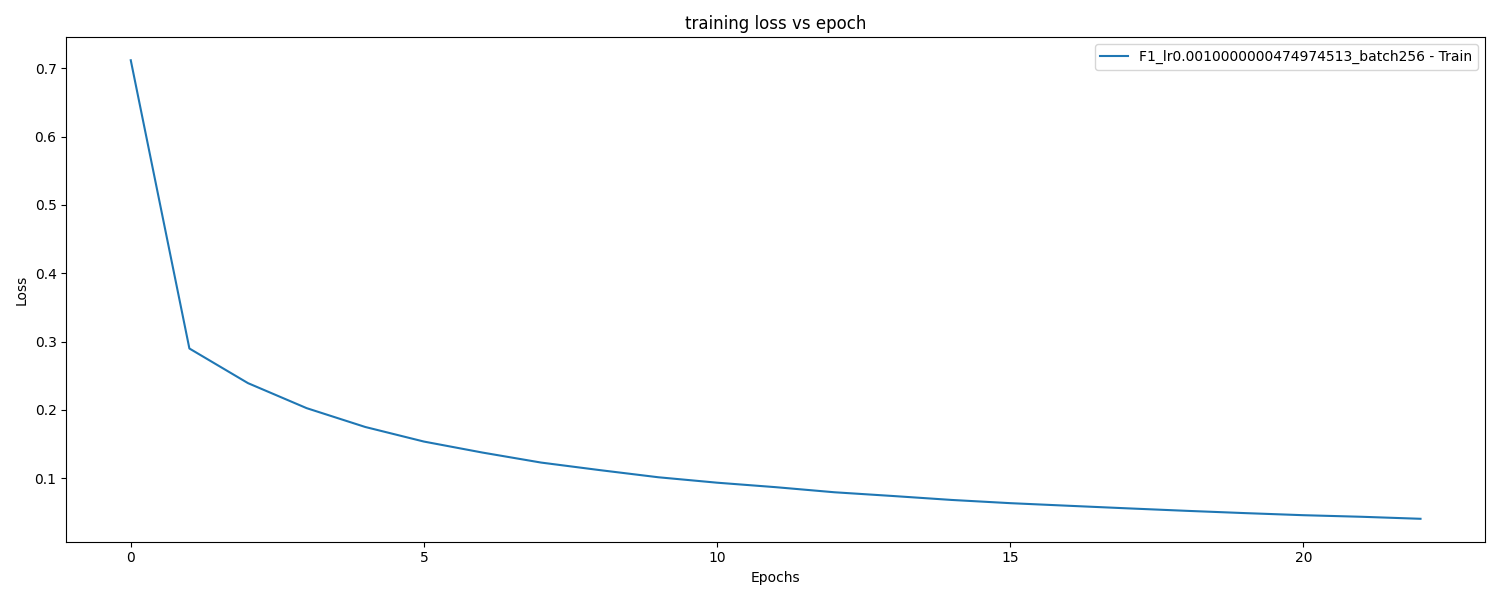
\includegraphics[width=1\linewidth]{f1_batch256.png}
    \caption*{f1 model, lr: 0.001, batch size:256,\\ 
    model: f1, test loss: 0.0879506, test accuracy: 0.9734, param size:50890}
\end{figure}
\subsection*{Part b}
\begin{figure}[!htbp]
    \centering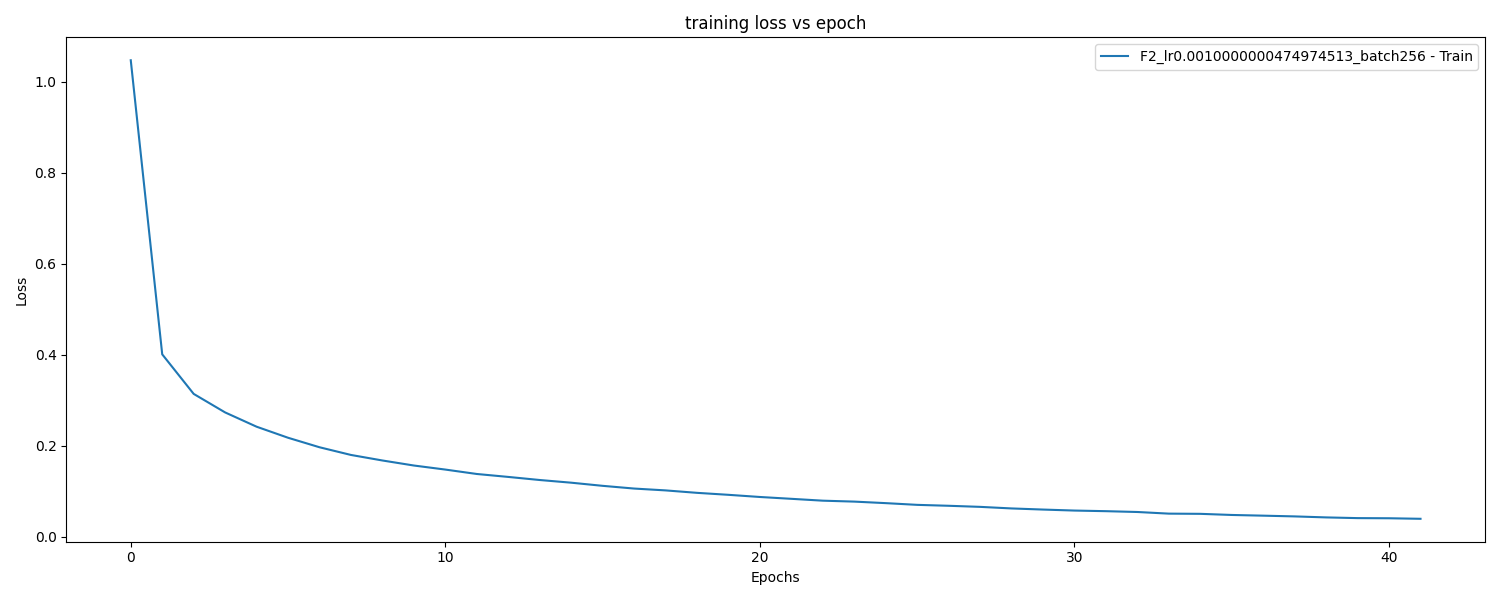
\includegraphics[width=1\linewidth]{F2_batch256.png}
    \caption*{f1 model, lr: 0.001, batch size:256,\\ 
    model: f2, test loss: 0.110278712, test accuracy: 0.9697, param size:26506}
\end{figure}
\subsection*{Part c}
model: f1, test loss: 0.0879506, test accuracy: 0.9734, param size:50890\\
model: f2, test loss: 0.1102787, test accuracy: 0.9697, param size:26506\\
\newline
Its really hard to compare which model is better given how similar the test accuracy is.
Although model f1 has slightly higher test accuracy, it also has larger number of parameters,
f2 achieve relatively close accuracy with only half of the parameters

\subsection*{code}
\inputminted{python3}{../homeworks/neural_network_mnist/main.py}